% =============================== 6. Q3 ===============================
\section{Question 3: Paying Riders to Move Bicycles}\label{sec:q3}

\subsection{What an incentive can and cannot do}

A truck can carry a bicycle ten kilometres. A rider can be persuaded to end a trip a
few hundred metres from where she intended, and no more: the reward would have to be
absurd to make someone ride across the city. The two instruments therefore operate at
different scales, and the right way to combine them is to ask how much of the
rebalancing problem each can absorb.

This fixes the unit of analysis. The deficit must be measured at the cell, in the hour
in which the cell loses bicycles, and the pool of candidate riders must be measured in
the same cell and the same hour. Measuring either over the whole day, as one is tempted
to do, inflates the pool by an order of magnitude and makes the incentive look free.

\subsection{The deficit to be absorbed}

For each cell $c$ let $n_{ct}=a_{ct}-d_{ct}$ be the net hourly flow and
\begin{equation}
\Delta_c \;=\; \max_t\left(0,\,-n_{ct}\right),
\qquad
N \;=\; \sum_c \Delta_c \;=\; 216{,}344 .
\label{eq:deficit}
\end{equation}
$\Delta_c$ is the number of bicycle-positions cell $c$ must receive during its own worst
hour to avoid drawing down its stock, and $N$ is the daily workload of a perfect
incentive scheme that ignored inventory. Of the 5{,}263 cells, 5{,}192 have $\Delta_c>0$;
the distribution is skewed, with median 17.9, 90th percentile 98.2 and 99th percentile
323.3 bicycles per hour.

\subsection{Will a rider accept?}

A rider whose trip is about to end at cell $j$ is offered $r$ CNY to end instead at
deficit cell $c$ at distance $d_{jc}$. The detour costs her the extra riding time plus
the extra walk,
\begin{equation}
\tau(d) \;=\; \frac{d}{v}\,\times 60 \;+\; \frac{1000\,d}{w}
\quad\text{minutes},\qquad v=10\ \text{km/h},\ w=80\ \text{m/min},
\label{eq:tau}
\end{equation}
and she accepts with the logit probability
\begin{equation}
\pi(d,r) \;=\; \frac{1}{1+\exp\left[-\left(\kappa r-\rho\,\tau(d)-c_0\right)\right]},
\qquad \kappa=2.0,\ \rho=0.35,\ c_0=0.8 .
\label{eq:logit}
\end{equation}
The parameters say that a rider values one yuan at two units of utility, one minute of
detour at 0.35 units, and carries 0.8 units of inertia against changing her plan. They
are not identified from our data --- no reward was offered in May 2017 --- and are
swept in Section~\ref{sec:sens}; what matters is the shape, not the level.

At the optimal reward derived below ($r=1.20$ CNY) acceptance falls from 78\% for a
50 m detour, through 54\% at 225 m, to 21\% at 450 m. The gradient is the whole story:
the scheme recruits the riders who were nearly going there anyway, and pays more and
more for the marginal ones.

\subsection{The supply curve of voluntary relocations}

Trips end at every distance in $[0,R]$, and the ones that end closest accept most
readily. We therefore discretise the catchment into six detour bands
$[0,50),[50,100),\dots,[300,450)$ m, count the trips $n_{cb}$ ending in band $b$
around cell $c$ during $c$'s deficit hour, and obtain the expected placements at
reward $r$ as
\begin{equation}
q(r) \;=\; \sum_c \min\left\{\Delta_c,\ \sum_b n_{cb}\,\pi(\bar d_b,r)\right\},
\label{eq:supply}
\end{equation}
where $\bar d_b$ is the band midpoint. The minimum enforces that a cell cannot absorb
more bicycles than it needs; the inner sum is the number of riders who would accept.
The function $q(r)$ is increasing and concave, and it saturates: no reward, however
large, can move a rider who is not there.

\begin{table}[htbp]
\centering
\caption[The supply curve at 450 m]{The supply curve at 450 m. ``Bill'' is $r\,q(r)$; the last column is the
marginal cost $\Delta(rq)/\Delta q$ over the interval since the previous row, to be
compared with the truck's 3.48 CNY.}
\label{tab:supply}
\small
\begin{tabular}{@{}rrrrr@{}}
\toprule
\textbf{Reward $r$ (CNY)} & \textbf{Placements $q$} & \textbf{Share of $N$} &
\textbf{Bill (CNY)} & \textbf{Marginal cost} \\
\midrule
0.2 & 51{,}380  & 23.7\% & 10{,}276  & --- \\
0.4 & 64{,}938  & 30.0\% & 25{,}975  & 1.16 \\
0.6 & 78{,}709  & 36.4\% & 47{,}226  & 1.54 \\
0.8 & 92{,}036  & 42.5\% & 73{,}629  & 1.98 \\
1.0 & 104{,}409 & 48.3\% & 104{,}409 & 2.49 \\
1.5 & 128{,}873 & 59.6\% & 193{,}310 & 3.63 \\
2.0 & 143{,}615 & 66.4\% & 287{,}229 & 6.37 \\
3.0 & 153{,}654 & 71.0\% & 460{,}961 & 17.31 \\
3.5 & 154{,}846 & 71.6\% & 541{,}961 & 67.95 \\
\bottomrule
\end{tabular}
\end{table}

\tabref{tab:supply} gives the curve. Two properties drive the recommendation.

\textbf{The first half is cheap.} The first 100{,}000 relocations cost 104{,}409 CNY,
an average of 1.0 CNY each, and at that scale the marginal placement still costs 2.5
CNY --- below the truck's 3.48, because there are enough riders passing within 100 m of
the deficit cells.

\textbf{The second half is not.} Beyond about 100{,}000 placements the cheap riders are
exhausted, and because the reward is uniform the platform must raise it for everyone in
order to recruit the few who are far away. The marginal cost of an extra placement then
rises faster than the reward itself: 3.63 CNY at $r=1.5$, 6.37 at $r=2.0$, 17.31 at
$r=3.0$. The curve ends in a wall at 71.6\%, where the pool of qualifying trips is
exhausted.

\subsection{The optimal mix}

The platform chooses $r$ to minimise the incentive bill plus the cost of moving the
residual by truck:
\begin{equation}
\min_{r\ge0}\ \ r\,q(r) \;+\; c_{\text{truck}}\left(N-q(r)\right),
\qquad c_{\text{truck}}=3.48\ \text{CNY}.
\label{eq:mix}
\end{equation}
The first-order condition is that the marginal cost of an incentive placement equals
the truck cost; on \tabref{tab:supply} that happens between $r=1.0$ and $r=1.5$. Solving
numerically gives
\begin{equation}
\boxed{\ r^*=1.20\ \text{CNY},\qquad q^*=115{,}385\ \text{placements}\ (53.3\%),\qquad
\text{bill}=138{,}462\ \text{CNY}\ }
\end{equation}
with a marginal cost of 3.46 CNY, within 1\% of the truck. The remaining 100{,}959
bicycles must be moved by truck for 351{,}116 CNY, so the daily cost is \textbf{489{,}578
CNY against 752{,}404 for an all-truck policy --- a saving of 34.9\%}
(\figref{fig:q3}c).

The optimum is not a corner solution, which is the useful part. Incentives do not
replace trucks; they remove the cheapest half of the trucks' work, and the two
instruments meet where their marginal costs are equal, as they should.

\subsection{Why the ceiling is physical}

At $r=3.5$ the scheme buys 71.6\% of the deficit and then stops. The remaining 28\%
is not a pricing failure: those cells have too few trips ending nearby in their deficit
hour for any reward to reach them. Widening the catchment helps only slowly
(\figref{fig:q3}d): 450 m covers 71.9\%, 600 m covers 83.3\%, 850 m covers 92.2\%, and
95\% requires a 1{,}025 m detour --- a walk of thirteen minutes, which no plausible
reward makes acceptable.

This is the correct division of labour between the instruments. Incentives should be
targeted at cells whose deficit is small relative to the traffic passing through them
--- the dense core, where a few hundred metres of redirection recruits thousands of
riders. Sparse peripheral cells, where the deficit is large and the passing traffic
thin, belong to the trucks.

\subsection{The scheme}

The mechanism that follows from the analysis has five elements.

\begin{enumerate}[leftmargin=1.6em]
\item \textbf{A uniform reward of 1.2 CNY}, paid on completion, credited to the
  account, and about the price of a ride. Uniformity matters: a personalised reward
  would extract more surplus but is perceived as unfair and invites gaming.
\item \textbf{A target set, not a target point.} The reward is offered for ending
  inside any cell in the current deficit list, recomputed hourly from the demand model
  of Section~\ref{sec:q1}. The list is exactly the set of cells with $\Delta_c$ above a
  threshold, which is what focuses the money where it is needed.
\item \textbf{A verified end.} The reward is paid only if the trip ends inside the
  electronic fence (Section~\ref{sec:q4}) of a target cell and the origin is outside
  it, which rules out the trivial strategy of riding in a circle.
\item \textbf{A daily cap} of three rewarded trips per user, which prevents a small
  number of users from absorbing the budget and keeps the scheme a broad-based nudge.
\item \textbf{A hard budget} of 140{,}000 CNY per day, which at $r=1.2$ is exactly the
  volume the analysis recommends; any surplus is carried to the next day.
\end{enumerate}

\begin{figure}[htbp]
\centering
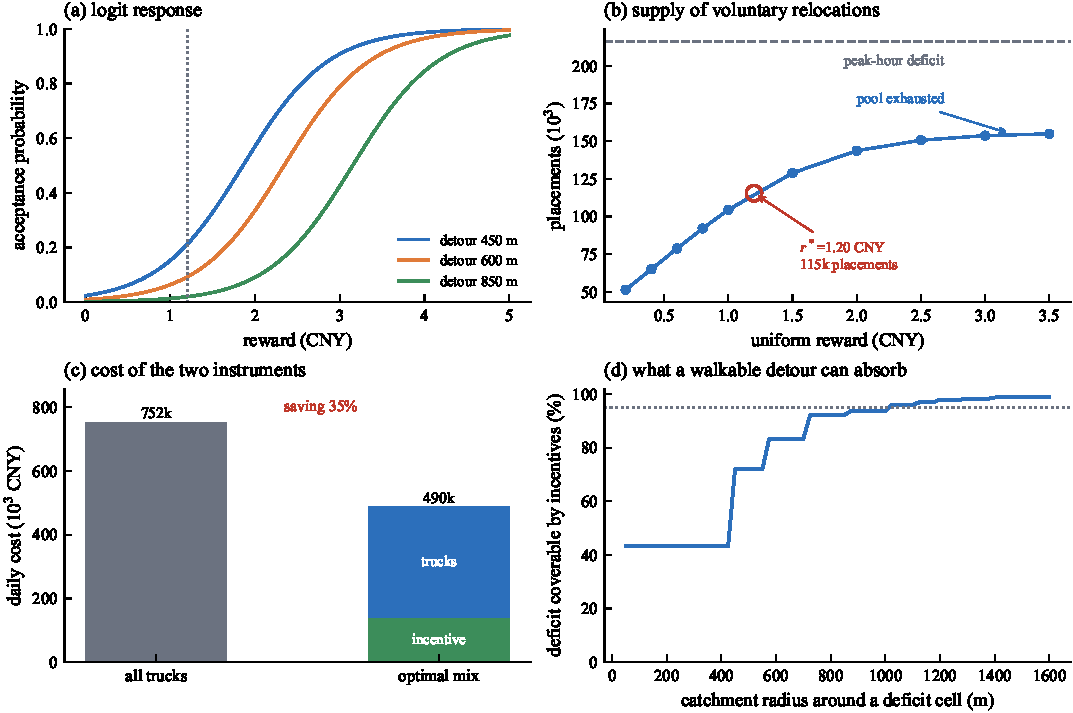
\includegraphics[width=0.9\linewidth]{../figs/fig5_q3.pdf}
\caption[Q3: acceptance, reward and savings]{Q3. (a) Acceptance probability against reward, for three detour distances.
(b) The supply curve of voluntary relocations; the dashed line is the peak-hour
deficit and the circle is the optimum. (c) Daily cost of an all-truck policy and of the
optimal mix. (d) Share of the deficit reachable within a catchment radius.}
\label{fig:q3}
\end{figure}
